\chapter{Introduction} \label{ch:intro}

\section{Description of study area}

The Great Smoky Mountains National Park (GRSM) which is located in the southern Appalachians spanning eastern Tennessee and western North Carolina is the second largest national park in the eastern united states.
It contains roughly 100 species of native trees, over 1,500 flowering plants, 200 species of birds, 66 types of mammals, 50 native fishes, 39 kinds of reptiles, and 43 species of amphibians.
This unique nature of the park has earned it the title of  International Biosphere Reserve by the United Nations \citep{NPS}.	
The GRSM is one the most visited parks in the US and its conservation is a high priority for the National Park Services (NPS) who look after it.		
Park conservation includes monitoring streams for the consequences of acid deposition.	
Acid deposition negatively affects the 3,000 km of streams present in the GRSM, impacting every living thing in the park which rely on the water quality in the park.  
	
\section{Acid Deposition and the GRSM}

Acid deposition is characterized as wet deposition (rain and snow), dry deposition (gases and particles), and fog or cloud deposition (occult).
These three weather modes transport and deposit the pollution of the industrialized world.
The top contributers of pollution to acid deposition are gas engines for transportation and industrial plants.
Power plants expel sulfur oxides (SO$_x$) and nitrogen oxides (NO$_x$) through smoke stacks high into the atmosphere where they react and fall to the earth as acid deposition.
The upper elevations of the GRSM receive some of the highest loading rates of acidifying nitrogen and sulfur species in North America \citep{johnson1992atmospheric}.  
Once the acid deposition constituents have entered in the environment they react with the surface waters, in the soil, and on man-made structures\citep{board1983acid}.  
This begins to acidify the surface waters which can harm any life forms that interact with it, including the soils as well as streams.
Along with adding acid to streams the added pollutants affect the alkalinity of water, or its ability to buffer a change in acidity,  and results in a pH change.  
As the pH level lowers, the ability of surface waters to sustain aquatic life also decline, this is called acidification. 
And while many factors affect the ability for the survival of aquatic life, acidification can be directly related to a lot of species survival.  

Acidification of bodies of water can be either chronic or episodic. 
Chronic acidification occurs when the body of water has constant low acid neutralizing capability (ANC); which creates a large area of  nearly un-inhabitable water where aquatic life would struggle to survive. 
Episodic acidification describes a rapid increase of acidity due to large surges of pollutants usually from snow melts or heavy rains.  
While chronic acidification may inhibit habitation, episodic acidification can kill aquatic life by quickly dropping the pH of streams.
A literature review in \citet{neff2009physiological} approximates a pH of 6 for negative biological effects and a pH of 5 for mortality for trout in the park.  
Stream pH levels between 5 to 6 can become toxic in the presence of aluminum through leaching and base cation exchange.
This toxicity can be harmful to eggs and fry in very soft waters in the lower end of the range \citep{robinson2008ph}.  

\section{The Stream Survey} 

The stream survey began as part of the park's Inventory and Monitoring program of the GRSM in 1993.
It collects grab samples multiple times per year from multiple sites in order to monitor the health of the streams in the park.
There are nearly 500 sites listed in the stream survey but the number of sites actually monitored has dwindled to the 43 sites used for this paper.
Currently, samples are collected from 32 sites every two months and an additional 11 samples are collected twice per year.  
These samples cover streams from 6 GRSM stream systems. 
Every sample is  measured for pH, ANC, conductivity, acid anions (CL$^-$,SO$_4^{2-}$,NO$_3^-$, ammonia (NH$_4^+$), the base cations (Ca$^{2+}$, Mg$^{2+}$, K$^+$, and Na$^+$), dissolved metals (Al, Cu, Fe, Mn, Si and Zn).  
A ManTech$^{TM}$ autotitrator was used for pH, ANC, and conductivity.  
A Dionex$^{TM}$ ion chromatograph (IC) was used for the analysis of CL$^-$, SO$_4^{2-}$, NO$_3^-$, and NH$_4^+$.  
A Thermo-Scientific$^{TM}$ Inductively Coupled Plasma - Atomic Emission Spectrometry (ICP-AES) was used for the study of Ca$^{2+}$, Mg$^{2+}$, Na$^+$, K$^+$, Al, Cu, Fe, Mn, Si and Zn.

\subsection{Database}

\begin{figure}[h!]
  \centering
  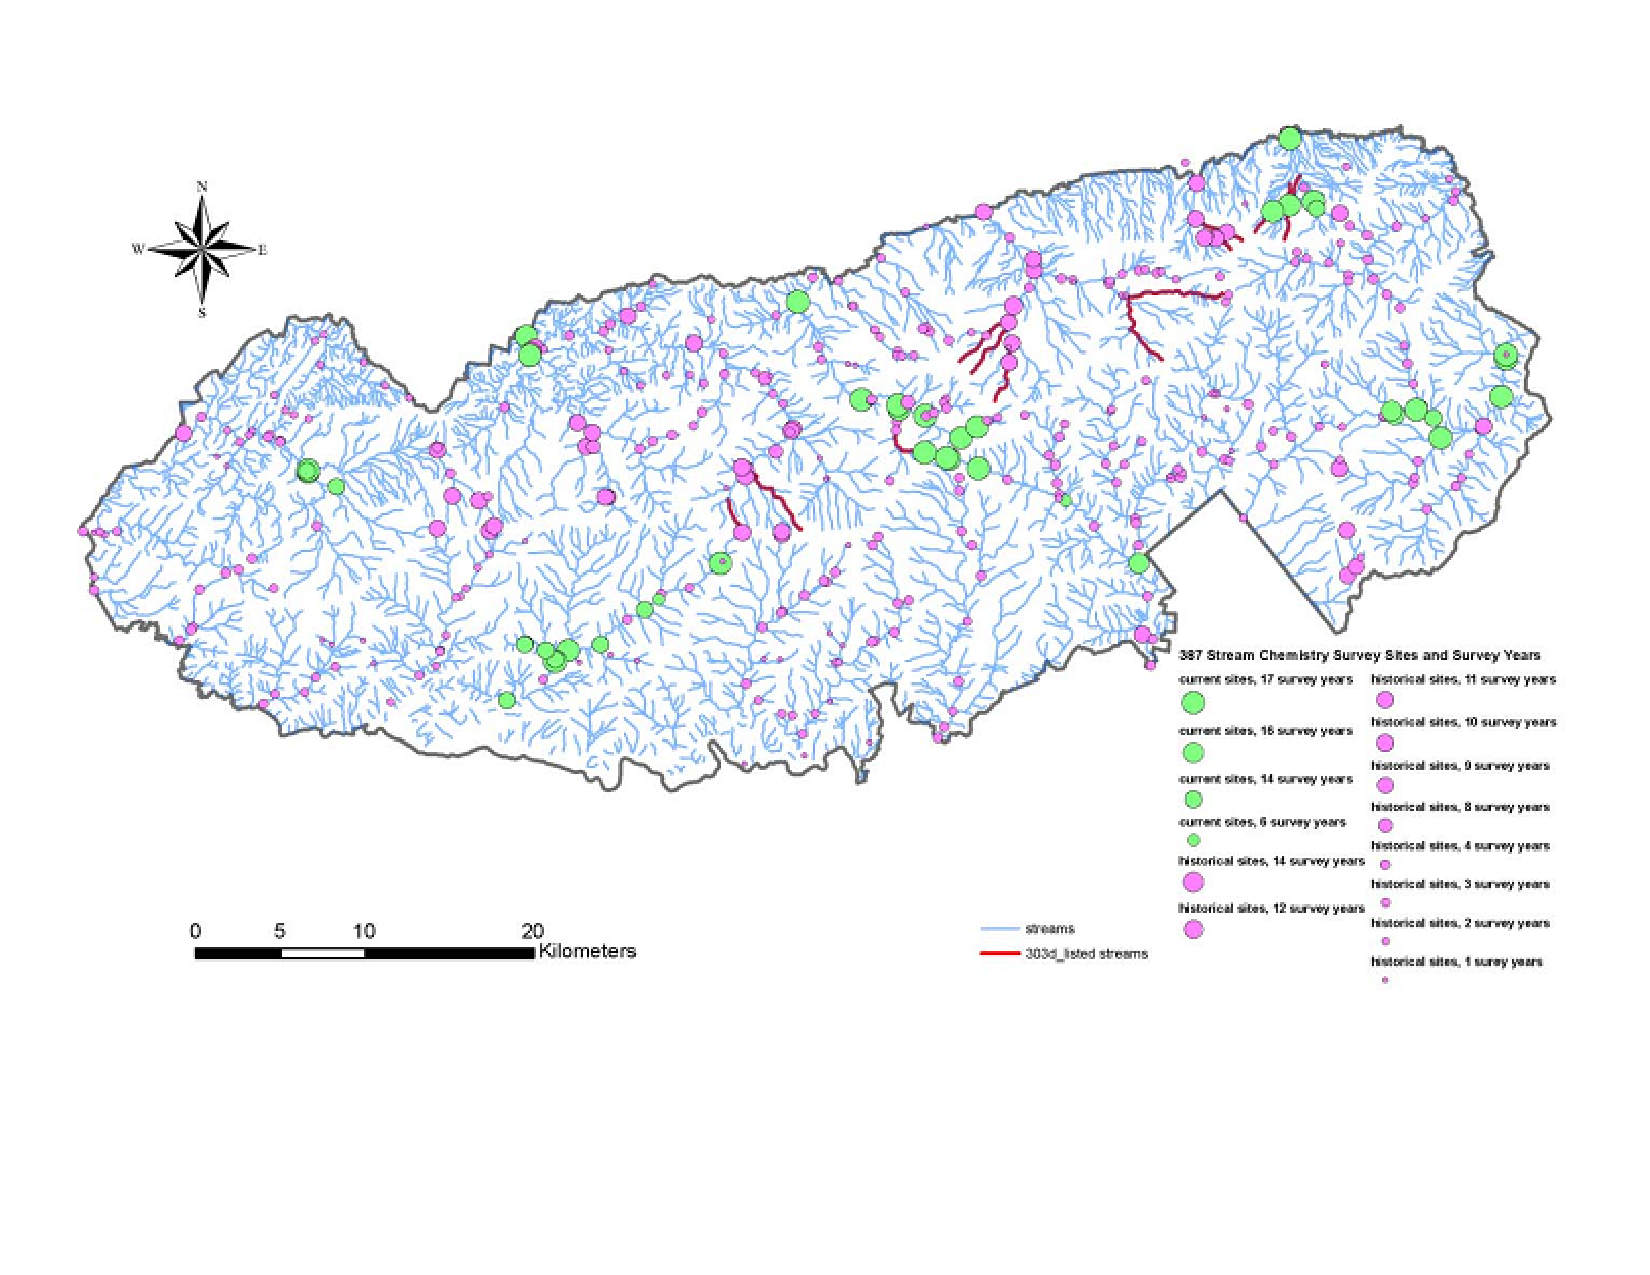
\includegraphics[width=6in]{SSsites}\\
  \caption{Site locations for the Stream Survey.  This map takes into account the years 1993 to 2009 so 3 more years need to be added to the current sites. }\label{fig:SSsites}
\end{figure}

All data is collected, under contract, for the NPS.
Sample data such as time, location, pH, and constituent concentrations are aggregated in spread sheets and formated to NPS specifications.
This data goes all the way back to the beginning of the survey in 1993.
Along with specific sample measurements each sample is labeled by its site ID, which indicates location.
Several important characteristics are known for each site such as stream name, geology, and elevation.

The database is dynamic and changes along with changes in the stream survey and lab methods.
Currently the collection, analysis, and formating falls under Dr.Schwartz of the University of Tennessee Civil and Environmental Engineering Department.
He inherited it from Dr. Robinson of the same department, who inherited it from the Forestry Department.
A difference in analysis and formating methods between the two departments is obvious in the data.
There are many more outliers present in the data curated by the Forestry Department which makes smoothing and statistically analyzing that half of the data harder.
In 2003 the survey changed from collecting grab samples from 90 sites to the current 43 sites \citep{odom2003}.
This makes the full database inconsistent and consistent data is important in statistical analysis.
Another inconsistency is the baseflow/stormflow classification which ends in 2010, while data up to 2012 will be analyzed here.
The baseflow/stormflow classification is useful when preparing the data for statistical analysis.

\subsection{Elevation Bands}

If the two most important location classifications for the survey data is site ID and stream system, then the third is elevation.
Elevation was found to be a dominant driver for predicting water quality among the park’s stream.  
Overall, results from the Biotics Effects report found that stream pH and ANC decreased at -.32 units and -35.73 μeq L-1 respectively, per 1,000-ft elevation gain \citep{cai2013}. 
This difference in pH due to elevation occurs because of many factors including occult deposition which effects the higher elevations greater.
Because pH decreases with an increase of elevation, elevation bands are used to characterize elevation.
Conductivity, chloride, and base cations were also found to significantly decrease with elevation gain.  
Sulfate showed no significant trend with elevation, however nitrate was found to significantly increase with elevation gain.  
The GRSM 2011 Annual Water Quality Report compared pH trend lines representing the current 43 sites from 1993-2010 with 2011.  
The data showed lines of similar slopes with different intercepts, which was interpreted to mean increasing pH at all elevations in GRSM streams.  
Acid deposition increases with elevation in the GRSM and the higher elevation streams would experience increased sulfate, and prolonged acidification if soil desorption becomes a dominant geochemical watershed process which could occur if pH increased to 6.0 and sulfate dropped below 50 μeq L-1 \citep{annualreport2012}.  
From a management perspective, the Biotic Effects Report contains limitations in the analyses to assess long-term changes because locations sampled have changed over time and most current sample locations are at lower elevations.

\begin{table}[htbp]
\centering
\begin{tabular}{ccccc}
\toprule
Elevation class & \multicolumn{1}{p{3cm}}{Range of elevation (ft) MSL} & \multicolumn{1}{p{3cm}}{Number of sampling sites} & \multicolumn{1}{p{2cm}}{Percent of NPS area*} & \multicolumn{1}{p{2cm}}{Percent of sampling sites} \\ 
\midrule
1 & $<$1000 & 0 &  & \\ 
2 & 1000-1500 & 7 & &  \\ 
3 & 1500-2000 & 13 &43.3 &65.0  \\ 
4 & 2000-2500 & 16 &  &  \\ 
5 & 2500-3000 & 18 & &  \\ \midrule
6 & 3000-3500 & 13 & 27.4 & 20.5 \\ 
7 & 3500-4000 & 4 & & \\ \midrule
8 & 4000-4500 & 5 & 21.2 & 12.1 \\ 
9 & 4500-5000 & 5 & &  \\ \midrule
10 & 5000-5500 & 1 &8.1 & 2.4 \\ 
11 & $>$5500 & 1 & &  \\ 
\bottomrule
\end{tabular}
\caption{Historical elevation bands for the 90 site survey. *Approximate percentages based on planimetering contour map}
\label{tab:Odomtable}
\end{table}


\begin{table}[htbp]

\begin{tabular}{cccc}
\toprule
Elevation class & Range of Elevation m(ft) & \multicolumn{1}{p{3cm}}{Number of sampling sites} &\multicolumn{1}{p{3cm}}{Percent of sampling sites} \\ 
\midrule
1 & $<$304.8 ($<$1000) & 0 &  \\ 
2 & 304.8-457.2 (1000-1500) & 4 &  \\ 
3 & 457.2-609.6 (1500-2000) & 4 & 67.4 \\ 
4 & 609.6-762 (2000-2500) & 9 &  \\ 
5 & 762-914.4 (2500-3000) & 12 & \\ 
\midrule
6 & 914.4-1066.8 (3000-3500) & 6 & 16.3 \\ 
7 & 1066.8-1219.2 (3500-4000) & 1 &  \\ 
\midrule
8 & 1219.2-1371.6 (4000-4500) & 3 & 14.0\\ 
9 & 1371.6-1524 (4500-5000) & 3 &  \\ 
\midrule
10 & $>$1524 ($>$5000) & 1 & 2.3\\ 
\bottomrule
\end{tabular}
\caption{Historical elevation bands for the 43 site survey}
\label{tab:43sitesurvey}
\end{table}


\autoref{tab:Odomtable} represents the concerns of Kenith Odom presented as table 38 in \citet{odom2003}.
This dissertation remodeled the survey from 90 sites to 43 and this table was used to suggest more high elevation sites.
The survey was reduced from 90 sites down to 43 but the elevational distribution was not fixed.
\autoref{tab:43sitesurvey} shows the percentage of sites per elevation bands for the 43 site survey just as \autoref{tab:Odomtable} does for the 90 site survey.
There is not much difference between the percentages.

\begin{figure}[h!]
  \centering
  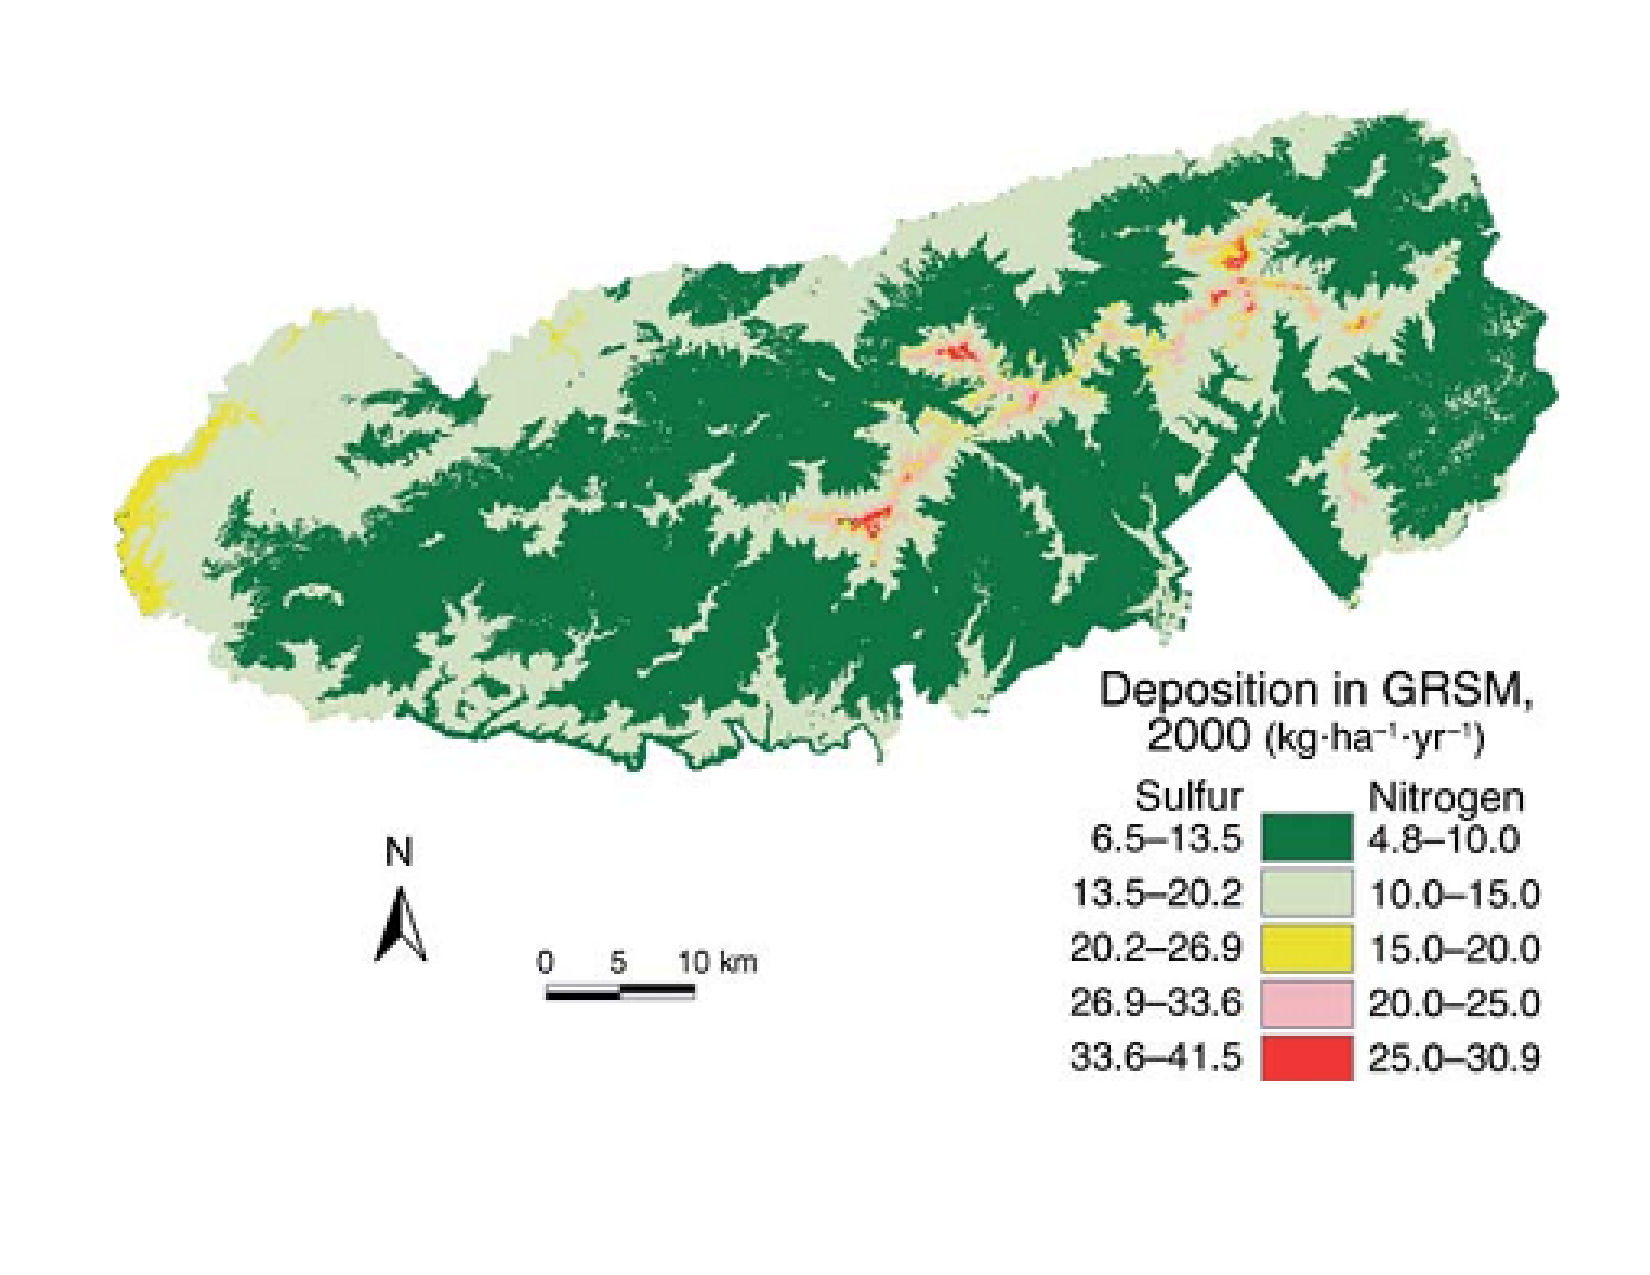
\includegraphics[width=6in]{DepositionHeat}\\
  \caption{ Modeled atmospheric deposition of N and S for the year 2000 and presented in \citet{weathers2006}.}\label{fig:depositionheat}
\end{figure}

For overall acidification of the GRSM, the high elevation bands could be the most important in the survey but they have the least amount of representation.
As can be seen in \autoref{fig:depositionheat}, which is a model, the highest deposition of sulfur and nitrogen is at the highest elevations.
Sites in these areas continue to receive low pH values in samples.
The tenth elevation class according to \autoref{tab:43sitesurvey} has only one site in it.
That whole elevation band is represented by only one spot in the GRSM and that is not very strong.

Without adding sites, the easiest way to fix this is to reorganize the elevation bands. 
For this paper the elevation bands were redesigned to try and strengthen the higher elevations.
A cluster analysis was explored for the task but it was not successful, there was to much variation to cluster by elevation only.

\begin{table}[htbp]
\caption{These elevation classes were created to add more weight to the higher elevations}
\begin{tabular}{clcp{5cm}}
\toprule
Elevation Classes & Meters (Feet)                              & n & Site \# \\ 
\midrule
1                        & 304.8-609.6 (1000-2000)           & 5   & 13 ,23, 24, 30, 479 \\ 
2                        & 609.6-762 (2000-2500)              & 9   & 4, 311, 268, 480, 310, 483, 147, 148, 484 \\ 
3                        & 762-914.4 (2500-3000)              & 13 & 114, 481, 482, 149, 66, 492, 137, 293, 270, 493, 485, 144, 224 \\ 
4                        & 914.4-1066.8 (3000-3500)         & 4   & 143, 142, 73, 71 \\ 
5                        & 1066.8-1371.6 (3500-4500)       & 4   & 74, 221, 251, 233 \\ 
6                        & $1371.6< (4500<)$                    & 2   & 253, 234 \\ 
\bottomrule
\end{tabular}
\label{tab:ElevationBands}
\end{table}

\autoref{tab:ElevationBands} contains all the sites of the 43 site survey not removed as outliers, so the 36 sites analyzed in this paper.
Each of the following statistical analyses will use these elevation bands to classify elevation for the stream survey data.

\section{Time sets}

Time trends are a common way to asses the health of the streams in the GRSM.
The analysis can be used for the current quality of the streams in the survey along with trends to determine where the quality is headed. 
Recently, trend analyses were conducted on the stream survey data in 2002 and published in \citet{robinson2008ph} and then again in 2009 for the Biotics Effects report \citep{cai2012}.
And even though these paper analyzed similar years (Robinson:1993-2002, Cai: 1993-2009), the results of these analyses are in disagreement.
Of the ten elevation bands analyzed in \citet{robinson2008ph} six had negative Julian date coefficients and the other four had no trend.
And the conclusion was reached that the pH is headed towards harmful and lethal conditions for aquatic life. 
In \citet{cai2012} of the 67 sites studied in the biotic effects report most showed no trend, 22 showed an increase in pH and 2 showed a decrease. 

The opposite trends reported in  \citet{robinson2008ph} and \citet{cai2012} suggest an inflection point in the trend line somewhere between 2002 and 2009. 
For this reason, and for easier comparison of results,  a separate data set will be partitioned off from 1993 to 2002 to equal the years analyzed in \citet{robinson2008ph}.  
A third data set will be partitioned after the year 2008 because this is the year that the Kingston and Bull run power plants installed scrubbers onto their smoke stack exhaust. 
The hypothesis being the SO$_4^{2-}$ concentrations will be noticeably different, and this difference could indicate a need for further study. 
These three time sets will be analyzed separately (1993-2002, 2003-2008, 2009-2012).

\section{Data smoothing}%put seasonality back into trend analysis
Water quality data is rarely perfectly formated for statistical analysis.
It is usually  non-parametric and can contain recording errors and other influential values \citep{helsel1992statistical}.
Four water quality variables will be used as dependents through out this paper: pH, ANC, NO$_3$, SO$_4$.
Each of these dependents are important for studying acid deposition: pH and ANC directly relate the health of the streams, NO$_3$ and SO$_4$ are the man-made pollutants thought to be causing increased acid deposition.
Before these variables can be used as dependents they need to be analyzed for distribution, outliers, cycles, missing values, and serial correlation\citep{helsel1992statistical}.
All of the dependent vectors had outliers, most of these were found as a part of the step-wise regression process which highlights influential data for further analysis.

The whole data smoothing process will not be shown here but pH will be shown as an example.
A figure of pH vs. month clearly shows seasonality which is important to address for trend analysis \citep{helsel1992statistical}.

\begin{figure}[h!]
\centering
	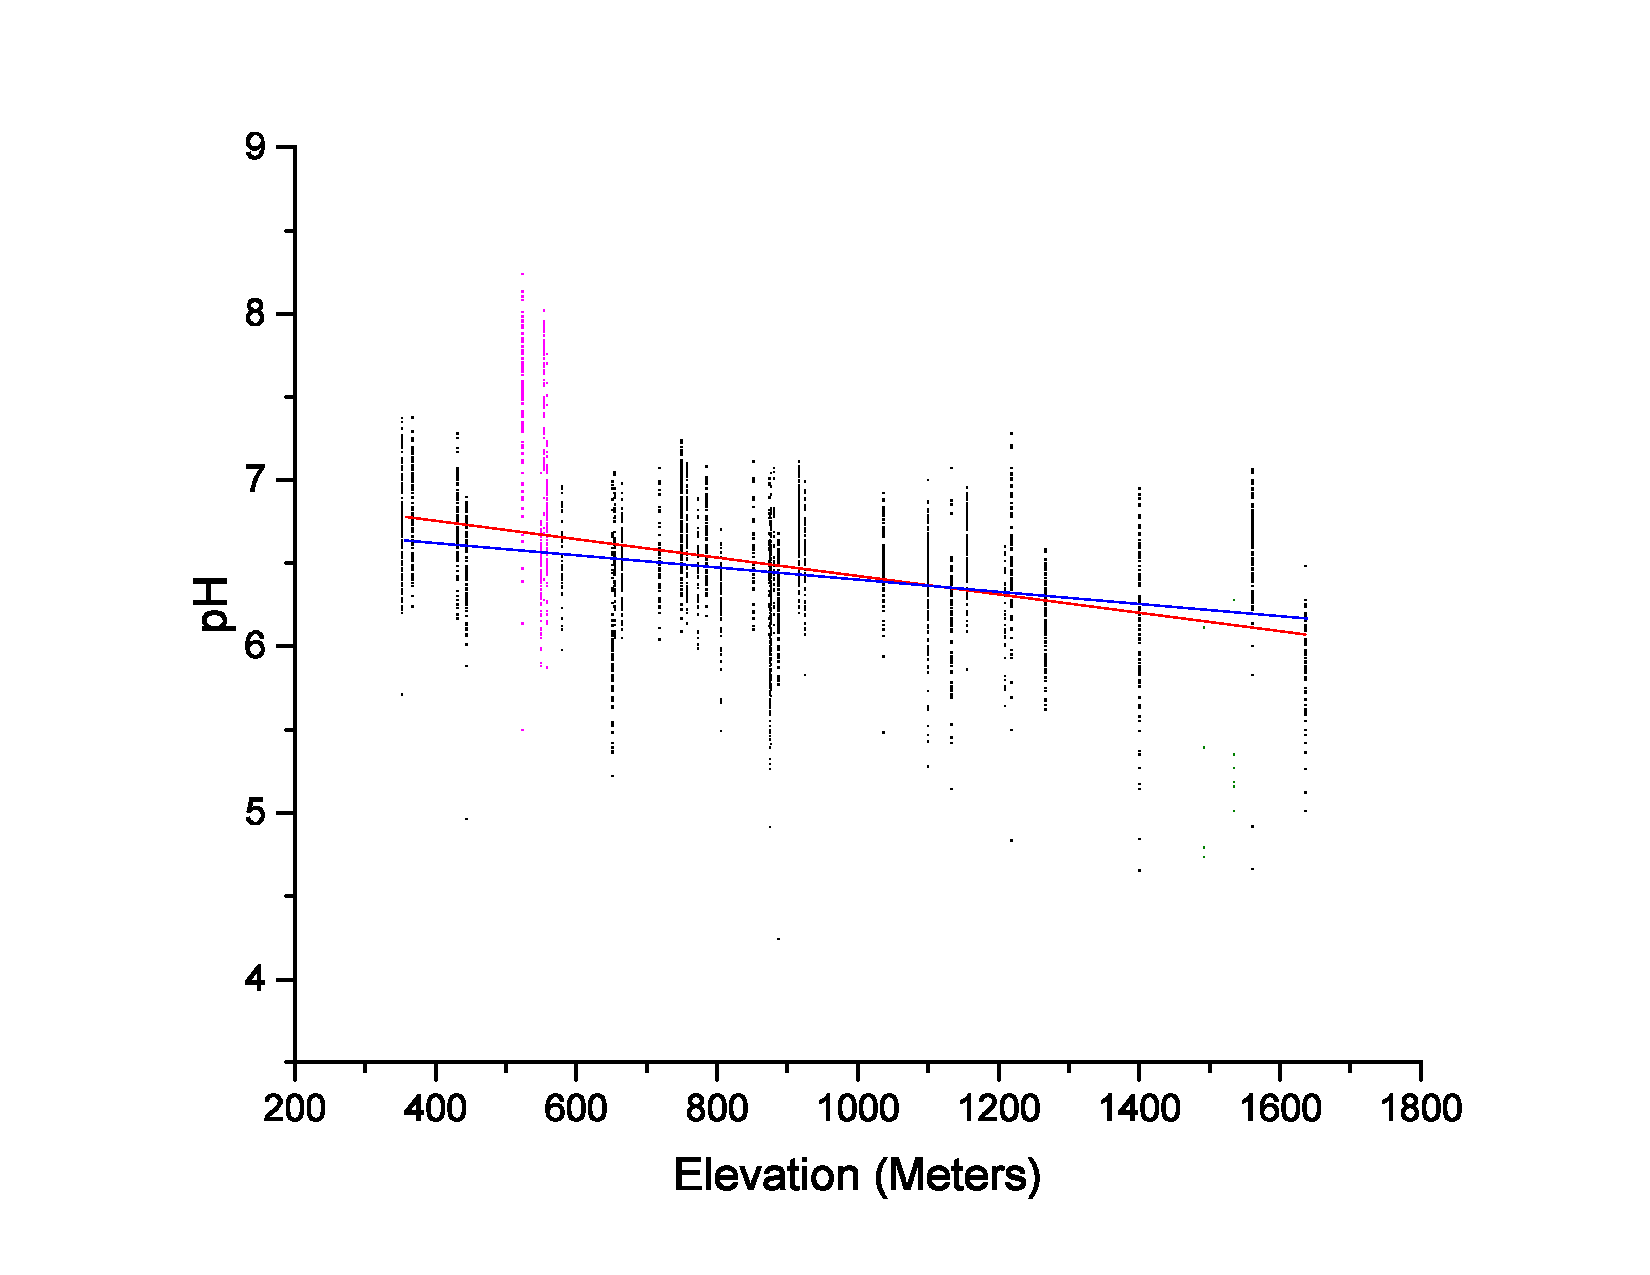
\includegraphics[width=6in]{pHdata}\\
	\caption{pH plotted vs. Elevation. With and without outliers.}
	\label{fig:pHdata}
\end{figure}

\autoref{fig:pHdata} shows the pH vs. elevation plot , which shows some outliers but also a negative trend in pH as elevation increases.
This graph contains two trend lines, one which represents the trend of all of the data points and the other represents the trend after the influential points are removed. 
Both of the trends are negative as elevation increases but the trend line containing the influential points is steeper. 

Much of the variance in \autoref{fig:pHdata} can be attributed to known influences in the stream survey data: Abrams creek watershed, sites that are affected by anakeesta geology, and stormflow \citep{neff2012influence}.  
Comparatively Abrams is a low elevation, low slope area where the underlying geology is Cades Sandstone, which buffers against acid rain very well. 
This sandstone contributes to high ANC values which in turn keep the mean pH levels higher than the rest of the sites in the survey. 
Site numbers 237 and 252 are sites which are down hill of road cuts that have exposed the underlying anakeesta formation to runoff.  
The anakeesta formation contains sulfidic slate ,which can have the same negative effect of acid deposition,  and keeps the pH values of streams very low.

Stormflow is both influential and detrimental  to GRSM water quality. 
Storms can bring high intensity rain fall which can very quickly reduce the pH and ANC of streams. 
In streams with low ANC and pH, episodic stream acidification can be harmful to aquatic life \citep{neff2009physiological}.  
Stormflow runoff can have a higher contribution to stream acidification than baseflow because it transports protons left in the upper layers of the soil by acid deposition. 
Stream acidification caused by stormflow can cause base cation exchange through the leaching of the surrounding soil. 
When the inherent base cation minerals run out, excess H$^+$ and Al will be released into the water. 
Increasing the H$^+$ concentration will lower the pH, and Al is toxic to biotics. 
Healthy streams can rebound to normal pH values; unhealthy streams can have permanently lowered ANC due to leaching.  
Measurements taken from stormflow can show uncharacteristically low pH values and high amounts of metals from leaching. 
In this way, stormflow is sometimes considered an influential group on the rest of the data, because the measurements are significantly different from the average. 
Dr. Cai characterized all of the available water quality data between 1993 and 2010 as storm flow or baseflow; this work is summarized in \citet{cai2013}. 
Water quality data after 2010 had not been characterized. 
If all stormflow observations are to be kept in the data, the years 2011 and 2012 would need to be characterized. 
Quick analyses were run to see how influential stormflow was on the data as a whole, and it turned out that some were and many were not. 
Instead of throwing out all of the stormflow observations at once, single influential observations could be explained by stormflow and removed. 
They can be removed on a case by case basis during the regression method.

\section{objectives}
Objectives of this study were to:
\begin{itemize}
\item  characterize time trends in stream pH and acidic anions among elevation ranges in order to assess whether conditions are improving or degrading, and to
\item characterize sampling variance based on available water quality data, within the context of time and elevation, to support development of the GRSM’s Vital Signs Monitoring Program.  The format of this thesis will follow these two objectives.  
\end{itemize}
\begin{itemize}
\item Has stream pH and acid anion concentrations changed among three time periods (1993-2002, 2003-2008, and 2009-2012), and among six elevation ranges (1000-2000ft, 2000-2500ft, 2500-3000ft, 3000-3500ft,3500-4500ft, 4500<)?
\begin{itemize}
\item Time trends
 \item Means Comparisons
\end{itemize}
\item What is the statistical power for water quality parameters based on frequency and elevational location?
\begin{itemize}
\item Post Hoc Analysis
\item A Priori Analysis
\end{itemize}
\end{itemize}
The thesis is organized into three separate chapters following the two above research questions. Each chapter will follow the technical format of introduction, methods, results, and discussion. 

%Increases in sulfate or nitrate in runoff and streams through acid deposition can cause an increase leaching of base cations, hydrogen ion, aluminum, and decreased ANC (Sullivan, 2004).  
%Leached aluminum can end up in streams and is toxic to fish (Driscoll 2003).  
%Rainfall and fog in the GRSM affect elevations above 4000 feet first higher elevations have steeper slopes which correlate to both thinner soils and base poor geology.  
%All these factors contribute to lower pH in higher elevations.  

%geology
%Stream acidification is more pronounced in higher elevation watersheds with underlying base-poor geology 
%(Herligy et al. 1991, Hyer et al. 1995; Wigington et al. 1996a,b).  

%episodic acidification
%Neff et al. (2013) observed this trend, but found other basin factors correlate to chronic and episodic acidification.  
%Other basins factors include drainage area size, vegetation, and soil properties, which factors all are change within an elevational gradient.  

%vital signs
%The National Park Service is currently developing a Vital Sign Monitoring Program for a number of national parks around the country, which includes the GRSM (Annual Administrative Report For Inventories and Vital Signs Monitoring FY 2010).  
%The goal of the GRSM Vital Sign Monitoring Program is to assess long-term changes in ecosystem health, including both terrestrial and aquatic environments. 
%In addition, the program will integrate these environments and and include existing data on basin factors associated with water quality.   

%data
%Although it is widely recognized that elevational gradient is important, a question about what elevation ranges are changing versus those that are not needs to be quantified in order to design an effective sampling program.  
%In addition, data must be collected at a set frequency to provide sufficient statistical power to make valid interpretations of change over time. 

 